\chapter{Implementação em VHDL}
\label{cap:implementacao}

\section{Arquitetura}

A ALU pode ser descrita funcionalmente em três blocos principais:
o caminho aritmético, a seleção do resultado e a geração das flags. Essa
divisão representa uma visão conceitual da arquitetura, enquanto a
implementação sintetizada apresentada na Figura~\ref{fig:blocos} detalha as
portas lógicas, os somadores e as redes de multiplexadores utilizados pelo
Quartus.

\begin{enumerate}
  \item \textbf{Caminho aritmético}: implementa um somador/subtrator de 8 bits
  compartilhado pelas operações ADDC, ADD, SUBC e SUB. O caminho é dividido em
  dois nibbles de quatro bits. O carry produzido pelo nibble inferior é
  encaminhado ao nibble superior e utilizado para determinar a flag de
  \textit{half carry} ou \textit{half borrow}. Nas subtrações, o operando B é
  invertido e o carry inicial é ajustado para produzir a subtração por
  complemento de dois;

  \item \textbf{Seleção do resultado}: combina os resultados das operações
  lógicas, aritméticas, de deslocamento e de rotação. A seleção é controlada
  por \texttt{op\_sel}. No código VHDL, essa função é descrita por uma
  atribuição \texttt{with-select}; durante a síntese, ela é implementada como
  uma rede de multiplexadores, conforme observado na Figura~\ref{fig:blocos};

  \item \textbf{Geração das flags}: calcula as flags a partir do resultado
  selecionado e da operação executada. A flag N é o bit mais significativo de
  \texttt{r\_out}, enquanto Z indica resultado nulo. A flag C recebe o carry ou
  borrow das operações aritméticas e o bit deslocado nas operações de
  deslocamento e rotação. As flags H e V são geradas pelo caminho aritmético e,
  nas operações em que não são definidas pela especificação, são fixadas em
  zero.
\end{enumerate}

\begin{figure}[htb]
  \centering
  \caption{Implementação sintetizada da ALU em portas lógicas,
  somadores e multiplexadores.}
  \label{fig:blocos}
  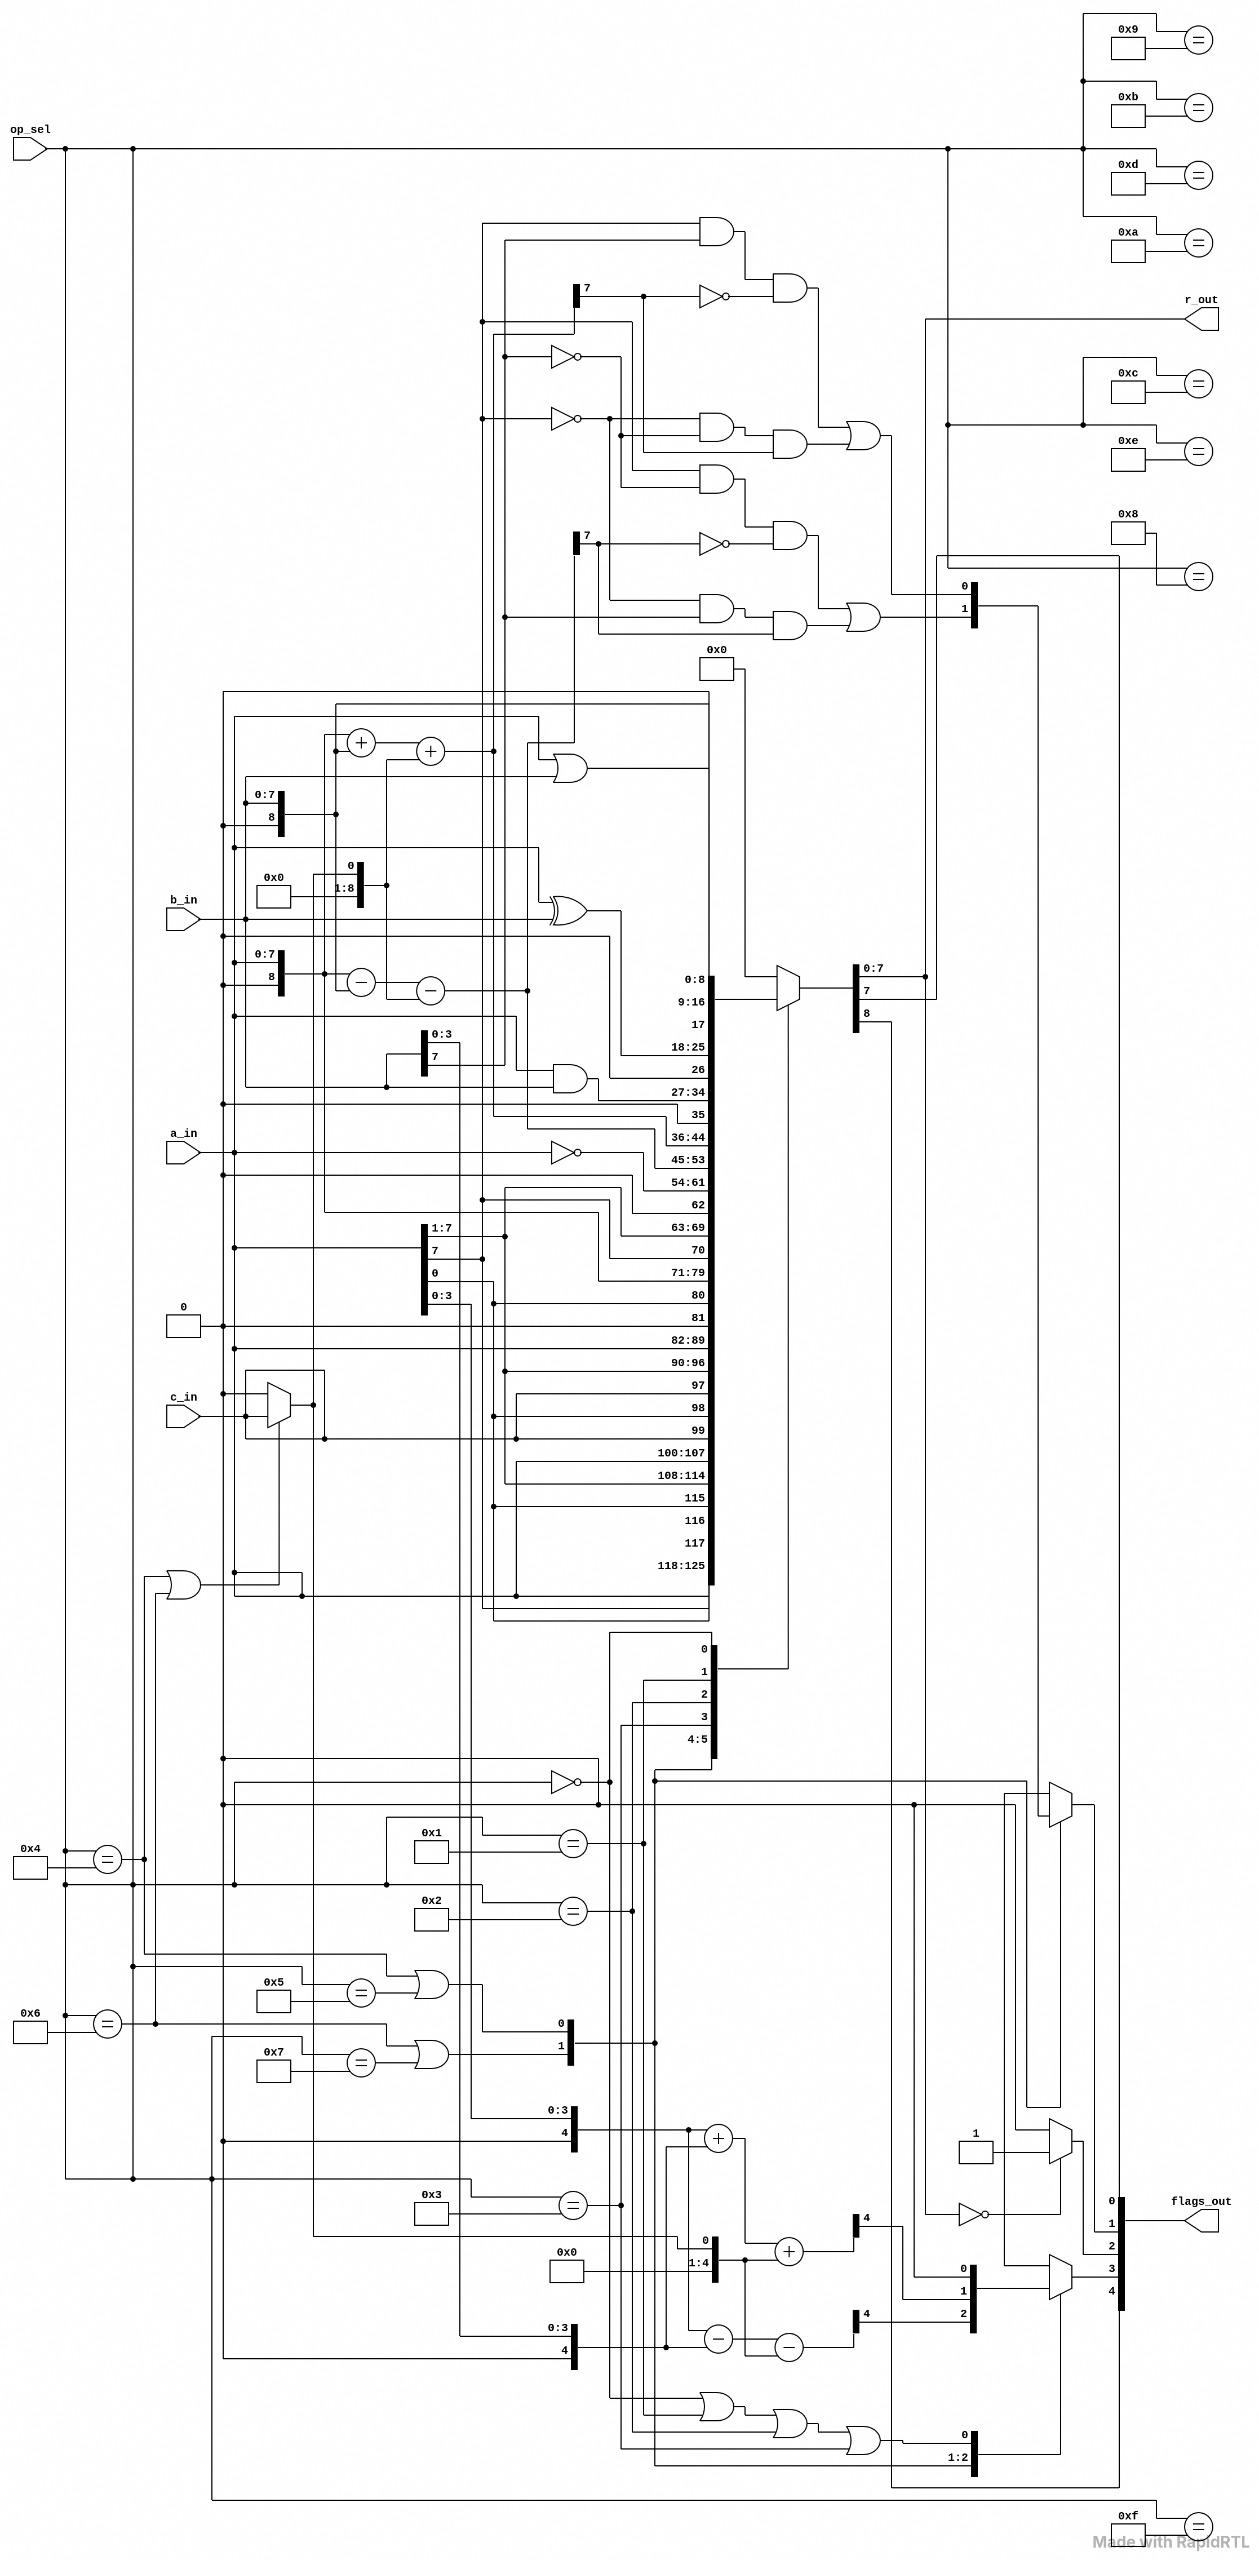
\includegraphics[
    width=0.95\textwidth,
    height=0.75\textheight,
    keepaspectratio
  ]{image/Portas-Logicas-Verticais.jpeg}
  \fonte{Elaborado a partir do site RapidRTL, utilizado como base o coigo fonte (alu.vhd).}
\end{figure}

\newpage
\section{Decisões de projeto}

\begin{itemize}
  \item \textbf{Subtração por soma}: usa-se a identidade da Equação~\ref{eq:sub}. O bit \texttt{op\_sel(1)} distingue subtração ($\texttt{1}$) de soma ($\texttt{0}$) e \texttt{op\_sel(0)} indica se o carry de entrada é usado (\texttt{0}). O carry de entrada do somador é
  \[
    c_{add} = \overline{s}\cdot\overline{op_0}\cdot c_{in} \;+\; s\cdot\overline{\overline{op_0}\cdot c_{in}},
  \]
  em que $s$ = \texttt{op\_sel(1)}.
  \item \textbf{Borrow}: em subtrações, C e H são o carry do somador invertido (XOR com $s$). Equação~\ref{eq:sub}.
  \item \textbf{Overflow}: calculado pela Equação~\ref{eq:ovf} usando o operando efetivo $b_{op}$.
  \item \textbf{\textit{Don't care}}: nas operações em que a especificação não define H ou V, essas flags são fixadas em `0', o que evita lógica desnecessária e saídas indefinidas na simulação.
\end{itemize}

\section{Código-fonte}

O Código~\ref{lst:alu} apresenta a entidade e a arquitetura completas, com comentários.

\lstinputlisting[
  style=vhdl,
  caption={Descrição VHDL da ALU (\texttt{alu.vhd}).},
  label={lst:alu},
  basicstyle=\ttfamily\scriptsize,
  breaklines=true,
  frame=single,
  extendedchars=true,
  literate={á}{{\'a}}1 {ã}{{\~a}}1 {ç}{{\c c}}1
            {é}{{\'e}}1 {ê}{{\^e}}1 {ó}{{\'o}}1 {õ}{{\~o}}1
]{vhdl/alu.vhd}
\vspace{-0.3cm}
\fonte{Autoria propria.}